\documentclass[titlepage]{article}
\usepackage{mathtools}
\usepackage{graphicx}
\graphicspath{{images/}}
\usepackage{titling}
\newcommand{\subtitle}[1]{%
  \posttitle{%
    \par\end{center}
    \begin{center}\large#1\end{center}
    \vskip0.5em}%
}

\title{Developer Guide}
\subtitle{The Header Importer Architecture}
\author{Mohammad R. Basirati}
 
\begin{document}
 
\maketitle
 
\tableofcontents
\newpage


\section{Introduction}
This document gives a complete description about how the tool header importer works. Furthermore it describes how to install needed tools for extending the importer. It assumes that you are familiar with lexical scanner, lexical parser and Jetbrains MPS\footnote{More information about MPS on https://www.jetbrains.com/mps/}.

Header Importer is a tool to import declarations from C headers into an mbeddr\footnote{More information about mbeddr on http://mbeddr.com/} project, so developers can use them in their code.

The process of importing a header file into an mbeddr project goes in three steps: 1. Scanning header files 2. Parsing scanner tokens 3. Importing declarations into mbeddr external module structure. We will discuss each step in detail in the following sections.

Step one and two work along in a Java project to prepare the required input for step three. The header importer tool Java project is located in folder bparser. The scanner generator produces lexer.java file and the parser generator produces two files: sym.java and parser.java. Lexer.java will tokenize the input file. Parser.java file can recognize the tokens by their identifier which has been defined in sym.java file. The last part of the Java project consists of classes which will be used to keep header file declarations. At the last stage, MPS importer gets the declarations and imports them into an mbeddr external module.

This document will explain each step of importing seperately: the scanner, the parser, and the MPS project. Then it will describe the details of every type of declaration in a C header. For every type of declaration, the document gives a brief definition, the parsing process, the importing process of parsed declarations into an mbeddr file, and finally the open issues. At last, there is a list of all open issues of the importer. 

\begin{center}

\begin{figure}[htbp]
\centering
\caption{Importing Process}

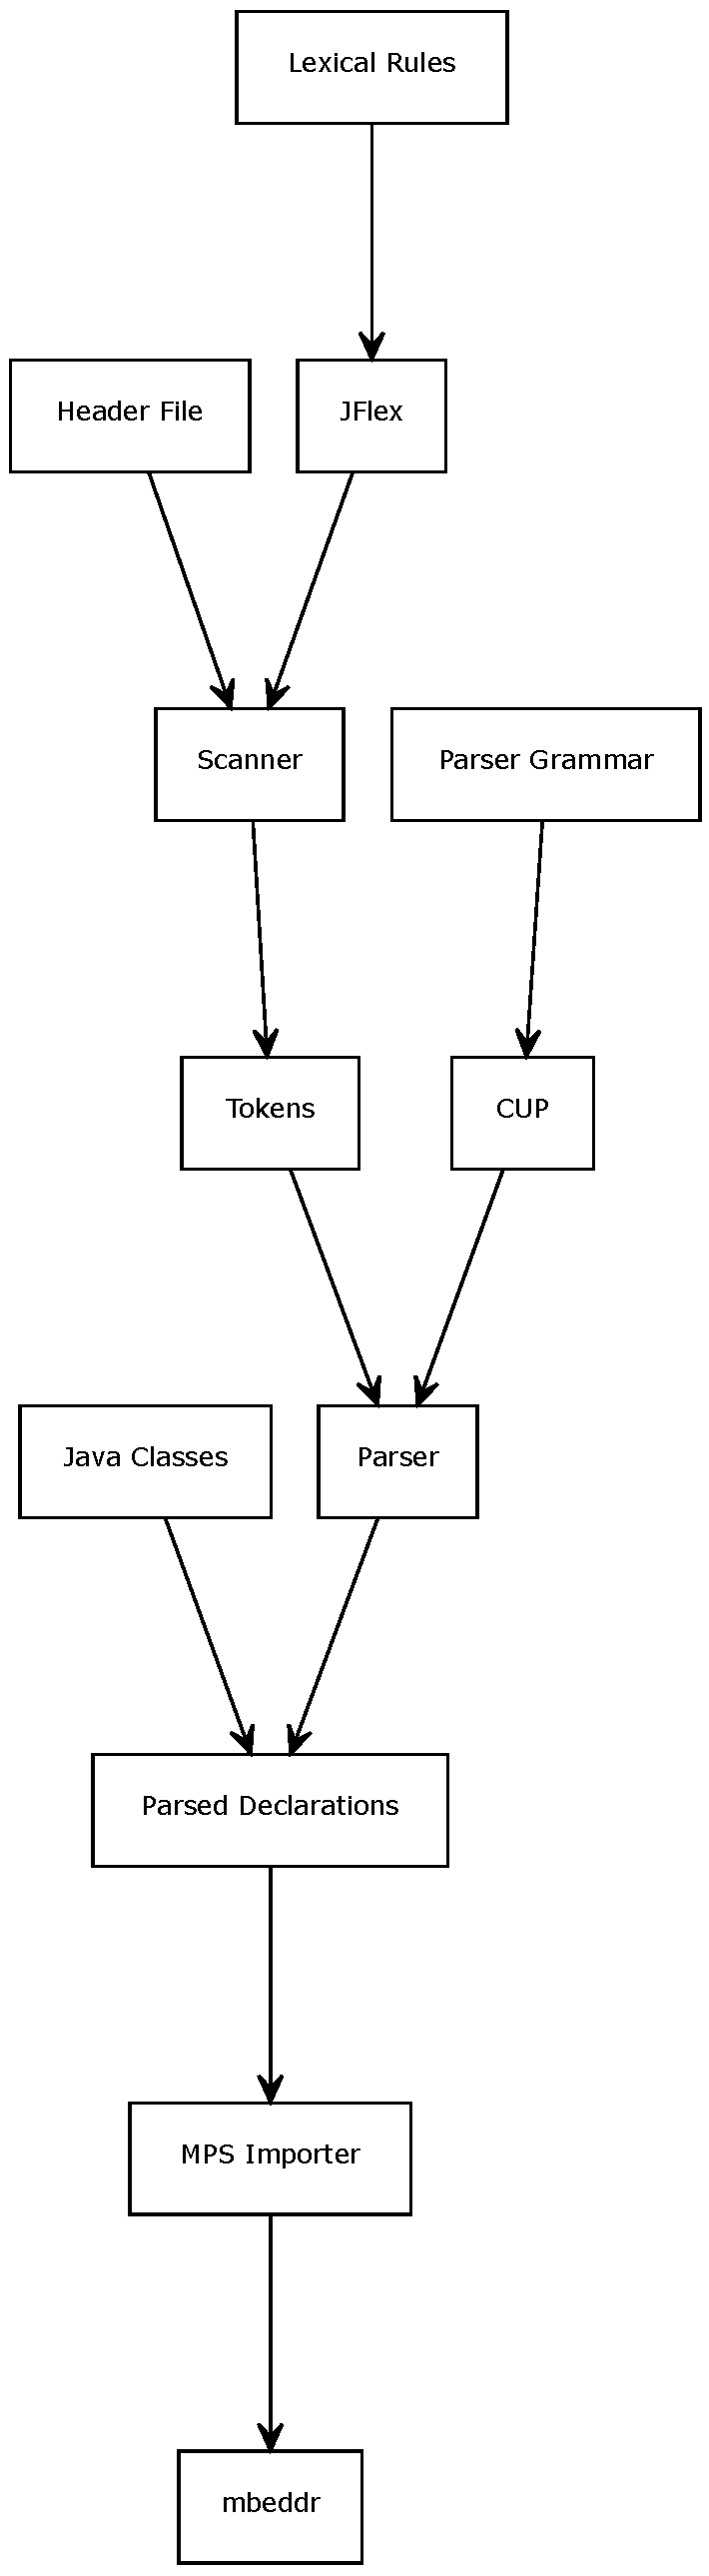
\includegraphics[scale=0.4]{process.pdf}

\end{figure}
\end{center}

\section{Scanner}
The first stage is to tokenize the header file. For this task the importer uses JFlex\footnote{JFlex Web Site http://jflex.de/} scanner. You can find the scanner files for the header importer inside the \texttt{"scanner\_parser"} folder. For compatibility issue of our tool over different versions of header files, we enhanced the scanner to be able to tokenize the gcc stdio.

\subsection{Installing JFlex Scanner}
All installation guides provided here are from  JFlex website installing guide\footnote{http://jflex.de/installing.html}. After downloading JFlex proceed as follows:

\emph{Windows:}
\begin{itemize}
\item Unzip the file you downloaded into the directory you want JFlex in.
\item Edit the file bin\textbackslash jflex.bat (e.g. ..\textbackslash jflex-1.6.1\textbackslash bin\textbackslash jflex.bat) such that

JAVA\_HOME contains the directory where your Java JDK is installed (for instance C:\textbackslash java)

and

JFLEX\_HOME the directory that contains JFlex (in the example: C:\textbackslash jflex-1.6.1)

\item Include the bin\textbackslash directory of JFlex in your path(the one that contains the start script, ..\textbackslash jflex-1.6.1\textbackslash bin). 
\end{itemize}

\emph{Mac/Unix:}
Using 'apt-get install jflex' should work OK, but in any case it didn't work, you can install it as follows:

\begin{itemize}
\item Decompress the archive into a directory of your choice with GNU tar, for instance to /usr/share:

tar -C /usr/share -xvzf jflex-1.6.1.tar.gz

\item Make a symbolic link from somewhere in your binary path to bin/jflex, for instance:

ln -s /usr/share/jflex-1.6.1/bin/jflex /usr/bin/jflex

If the Java interpreter is not in your binary path, you need to supply its location in the script bin/jflex.
\end{itemize}

After installation you could be enable to run JFlex. The simplest way to run JFlex without any option is:

jflex THE\_SCANNER\_FILE.jflex

\subsection{The Scanner Structure}
The scanner has three states which can identify one line comments, multiple lines comments, and strings. All the charachter sequences tokens that the scanner returns consists of: all possible operators in c, define, undef, if, ifdef, ifndef, else, endif, include, extern, pragma, typedef, struct, all c types (int, char, etc.), numbers , and identifiers.

The scanner can recognize the compiler preprocessing words which begin with double underscore and returns the token COMPWORD for them. Other compiler preprocessing phrases will be ignored by the scanner.

The lines that begin with define keyword for declaring macros and constants, scanner returns the whole line to the parser and doesn't tokenize their expression. In the parser section we will discuss this issue in detail.


\section{Parser}
The parser has been generated by CUP\footnote{CUP Web Site http://www2.cs.tum.edu/projects/cup/}. JFlex scanner is designed to work along with CUP. Basically the parser gets tokens from the scanner and matches them by the grammers which are defined in .cup file. The parser files of header importer located in \texttt{"scanner\_parser"} folder.

\subsection{CUP Parser Installation}
All installation guides provided here are from  CUP website installing guide\footnote{http://www2.cs.tum.edu/projects/cup/install.php}. After downloading CUP proceed as follows:

CUP comes with a generator part and a runtime part. Working with CUP comprises two phases:

\begin{itemize}
\item[Parser generation]
Parser generation is done by creating a .cup file, that represents a parser specification. These specifications need to be processed by the parser generator. For this end, you should place java-cup-11a.jar besides the your\_parser.cup file and run this command: 

java -classpath java-cup-11a.jar java\_cup.Main < your\_parser.cup

This will create the corresponding parser as a .java file, that can be integrated into Java projects as usual.

\item[Parser runtime]
During parser runtime, the generated parser needs a few classes, on which it is dependent. These classes are contained in the java-cup-11b-runtime.jar file. This Java package needs to be included into the target project's classpath. The original generator package java-cup-11b.jar however does not need to be distributed alongside the target project.

\end{itemize}





\subsection{The Parser Structure}
The grammer of the parser consists of two main parts: preprocessing steps and general declarations. Preprocessing steps comprise of the define, if, ifdef, ifndef, else, endif, include, and COMPWORD token that is the token returned by scanner for preprocessing words used by compilers.

\textbf{program ::= program code\_part \textbar code\_part;}

\textbf{code\_part ::= pre\_process\_step \textbar general\_declaration SEMI \textbar EXTERN general\_declaration SEMI \textbar error;}

General declaration part, consists of 4 type of declaration: typedef declaration, struct declaration, variable declaration, and function prototype declaration.

\subsection{Declaration Classes}
The IDEA Java project\footnote{Intelij IDEA Web Site https://www.jetbrains.com/idea/} has several classes for managing and keeping the declarations. These classes are used by parser to define declarations and used by MPS importer part to get the declarations and import them into an mbeddr module. Descriptions for each class and how they colaborate in the parsing phase are described blow:

\begin{itemize}
\item[CodeGenerator]
CodeGenerator class is responsible for being a proxy between the parser and MPS part. The parser export parsed declarations by calling CodeGenerator methods.On the other hand, the MPS part gets the declarations from CodeGenerator list of all declarations. Besides, CodeGenerator class has the responsibility of taking care of if blocks and structs.
\item[Declaration]
Declaration is an abstract class which all other classes execpt for CodeGenerator, extend it.
\item[ConditionalBlock]
This class is used for defining conditional directives(e.g. \#ifdef) blocks. It has two lists of declarations: true block and false block.
\item[Define]
It is used for define declarations(constants and macros).
\item[Function]
It keeps the information for function declarations and function pointers. It has a list of parameters, a return type, and a name. 
\item[Variable]
It defines a variable declaration.
\item[Struct]
It has a list of struct declarations and a name.
\item[Typedef]
It defines a typedef declaration.
\item[Include]
It holds a name for what should be included.
\end{itemize}

\section{MPS Importer Project}

\subsection{Installing MPS}
For installing MPS you just need to download it from MPS website download page \footnote{https://www.jetbrains.com/mps/download/index.html} and unpack it.

\subsection{The MPS Part Structure}
The MPS project part has five main classes:
\begin{itemize}
\item[ParserAdapter] ParserAdapter initiates a new java Parser class and parses the given file address. It returns the CodeGenerator class as the result which has all the parsed declarations.
\item[Importer] The importer class coordinates all the process of importing a parsed header file into the mbeddr like creating a new SupportVariability file, adding needed references to the modules, etc.
\item[ImporterCore] The ImporterCore class is responsible to add declarations based on their types(struct, function prototype, etc.) to an mbeddr module.
\item[VariabilityImporter] The VariabilityImporter class provides all needed functions to handle conditional directives in the variability mechanism of the mbeddr.
\item[Tyeper] The Typer class is responsible for managing the types in mbeddr. It creates new user defined types(e.g. structs, typedefs, etc.) and keeps the track of existing types in an mbeddr module.
\end{itemize}


\section{Integrating Scanner, Parser, and MPS Project}
Generally the generated scanner and parser java files should be included in a java project. The importer has these files in bparser IDEA java project to work with each other. There are three files: lexer.java, parser.java, and sym.java. Besides the bparser project consists of other needed java classes for handling the import process. Then the bparser .jar file should be included in the MPS project.

\section{Structs and Unions}
\subsection{Background}
Header files can have definitions of structs and unions. Structures and unions are defined exactly with the same syntax. The difference between a struct and a union is the way C stores them. A struct is a record structure and each member in the struct is allocated a new space, while for a union only one chunk of memory is allocated for all its members. Therefore writing to a struct member changes only the value of the member written to, while writing to a member of an union will render the value of all other members invalid. 
\subsection{Overview on Importer Implementation}
Since struct and union definition has exactly the same syntax, so the way importer treats them is exactly the same and both are kept in a same java class.
\subsection{Parsing Structs and Unions}
The scanner identifies the 'struct' and 'union' tokens and returns their corresponding tokens to the parser. Struct and union definition is under general declaration part of the parser. Every struct and union has an id and a body of declarations. The body part can have variable declarations and preprocessing steps(e.g. conditional directives). 

Structs and unions are both kept in a java class called 'Struct'. The struct class keeps a list of declarations of a struct or an union memebrs, an id, and a boolean attribute 'isUnion' which defines whetere class belongs to a struct or an union.
\subsection{Importing Parsed Structs and Unions to mbeddr}
The process of importing structs and unions to mbeddr is straight forward, as mbeddr has these concepts completely. 


\section{Typedefs}
\subsection{Background}
Typedefs are used to declare new names for existing types. These typedef names are aliases for existing types, and are not declarations of new types and cannot change the meaning of an existing type.
\subsection{Overview on Importer Implementation}
The hard task in importing a typedef is at parsing phase as the typedefs can have very complex expressions. The rest of the process is straight forward, a java class is responsible for keeping the typedef information: a typedef-name and a existing type. Right now the importer can import typedefs with only one pair of typedef-name and existing type. The existing type can be any basic types, pointers, structs, unions, and enums. If there is a more complicated type definition, the importer will fail to import it.
\subsection{Parsing Typedefs}
The scanner identifies typedef keyword and returns a token to the parser. The parser count a typedef as its general declarations. A typedef expression is expected to be a TYPEDEF token followin a general variable declaration, a struct definition or type, or an enum declaration.

The information of a typedef is saved in a java class called 'Typedef'. A boolean attribute called 'isStruct' defines whetere a typedef is defining a new struct or not. 
\subsection{Importing Parsed Typedefs to mbeddr}
The process of importing typedefs to mbeddr is straight forward, as mbeddr has this concept completely. 
\subsection{Open Issues}
\begin{itemize}
\item \emph{Parsing Typedef Expressions:} The importer now lacks parsing all possible typedef expressions and the parser part needs to be improved in future.
\end{itemize}


\section{Variable Declarations}
\subsection{Background}
Every variable in C has a unique name and a type. A variable is a name given to a some location in memory that holds a value which the program can manipulate it. 
\subsection{Overview on Importer Implementation}
The importer can recognize all basic variable types: char, int, float, double, short, short int, long, long int, long long, long long int, long double. Moreover the importer can recognize all possible more complicated types: pointers, function pointers,signed and unsigned types, and arrays. The user defined types like structs, unions and typedefs are supported by the importer too.
\subsection{Parsing Variables Declarations}
The scanner recognizes all basic variabe types and returns a symbol for each of them. The importer can handle pointers, signed and unsigned types, and arrays. A char sequence can be recognized by the parser as a user defined type.
\subsection{Importing Parsed Variable Declarations to mbeddr}
The importer has a class called 'Typer' which crates new types based on parsed types. Besides this class is responsible for recognizing predefined types in a header file. For example if there is a typedef, the Typer class could be able to identify the typedef's name as a new type, but there are some situations which the importer cannot import a typedef because of inability to parse it completely. In those situations, in the rest of the header file, the Typer class will not recognize the new type name defined by the typedef, so the importer will add a new typedef with the corresponding type name and put \emph{void*} as the type.

In general the importer will import all the variable types and if there is a type which is a user defined type, but the importer cannot recognize it, the importer adds a new typedef with that type's name and put \emph{void*} as the type. 

\section{Function Prototypes}
\subsection{Background}
A function prototype declaration specifies name of the function, the return type and type of the arguments, but it lacks the function body. In a function prototype, arguments' names are optional.
\subsection{Overview on Importer Implementation}
The importer identifies function prototypes and import them to mbeddr. The types used in a function prototype are imported into mbeddr with the same mechanism of variable declaration types.
\subsection{Parsing Function Prototypes}
The scanner identifies different parts of a function prototype seperately and returns its corresponding token to the parser. Function prototypes are considered as the general declarations of the parser. Every function prototype has a type, aname and a parameters part which is surrounded by paranthesis. The parameters part are only types seperated by commas.
\subsection{Importing Parsed Function Prototypes to mbeddr}
If there is a type in defining a function prototype which is missing for any reason, the imported adds  a new typedef with the name of that type and \emph{void*} as the type. The mechanism of importing types is exactly the same as importing variable declarations.

In mbeddr is necessary that arguments have names, so the importer adds a name for them sequentially(e.g. p0, p1, p2, ...).
\subsection{Open Issues}
\begin{itemize}
\item \emph{Parsing Arguments' Names:} Right now the importer's parser cannot parse the function prototypes which their arguments have names as an option. The parser should be improved in future works.
\end{itemize}

\section{Constants and Macros}
\subsection{Background}
Constants and macros are defined by \#define directive. By defining a constant, whenever the identifier name of the constant shows up in the file, it will be replaced by its corresponding value. Macro is the association of an identifier or parameterized identifier with a token string. After the macro is defined, the compiler can substitute the token string for each occurrence of the identifier in the source file.
\subsection{Overview on Importer Implementation}
A \#define statement consists of two part: 1. an identifier which can be parametrized(in case of macro) 2. a value. In mbeddr mechanism, the correct declaration of the identifier part is mandatory for using it in an 'Implementation Module', but it's not necessary to declare the corresponding value part, as it will be linked from the original C header file later. Therfore importing constants and macros doesn't need importing of the exact value's expression. The importer parses the identifier part and import it as a constant or macro to mbeddr and leave the value part as an empty string.
\subsection{Parsing \#define Directives}
JFlex scanner identifies \#define directive and it returns the 'DEFINE' symbole to the parser and the exact text of its line.

The \#define directive is parsed as a preprocess step. The parser creates a new instance of a java class called 'Define'. Define class has a function 'declareDefine' which extract the identifier part of the \#define directive and saves it in the class' attributes.

\subsection{Importing Parsed \#define Directives to mbeddr}
The importer defines a macro or a constant(in mbeddr \#constant or \#alias) with its corresponding identifier. If the value of a constant is integer, it will be imported, but if it's an expression or a non-integer(e.g. string), it will be imported as a string. Mbeddr will use the original C header file at the build time, so importing the value part is not necessary.
\subsection{Open Issues}
\begin{itemize}
\item \emph{Importing Correct Values:} Importing the correct value parts of constants and macros can be a future work.
\end{itemize}

\section{Preprocessor Conditional Directives}
\subsection{Background}
A conditional directive instructs the preprocessor to select whether or not to include a chunk of code in the final token stream passed to the compiler. Preprocessor conditionals can test arithmetic expressions, or whether a name is defined as a macro, or both simultaneously using the special defined operator. Conditional directives are: \#ifdef, \#ifndef, \#if, \#else, \#elif, \#endif.
\subsection{Overview on Importer Implementation}
Importing conditional direcrtives is one of the hardest task in importing a header file. Mbeddr doesn't support conditional directives, so the implementation of importer used mbeddr's abilities in a creative way. Conditional directive are transalted to 'Feature's in mbeddr and each import makes a unique 'VariabilitySupport' file that holds all conditional directives information as mbeddr features. Then each line of declarations in External Module file of mbeddr, has a 'Presence Condition' which defines this declaration is under which feature, i.e. conditional directive, of previously automatically created VariabilitySupport file.
\subsection{Parsing Conditional Directives}
JFlex scanner identifies \#if, \#ifdef, and \#ifndef directives by a JFlex expression which ignores the whole rest of line front of them and returns a token IF, IFDEF, or IFNDEF to parser with the correspanding exact text of their line. For \#else and \#endif tokens, scanner returns ELSE and ENDIF respectively by identifying the exact text 'else' and 'endif'. The sharp sign \# itself is recognized as a different symbole seperately.

All conditional directives are parsed as a preprocess step. IF, IFDEF, and IFNDEF tokens initiates a new class in java called 'ConditionalBlock' which handles the information of a conditional directive. ConditionalBlock keeps a list of all decelaration under it and its corresponding else block. Each ConditionalBlock has a boolean attribute called 'condition' which identifies that we are on if block or else.

Conditional directives can have complex arithmetic and logical expressions, so the parsing phase could get problematic. Since the importer's implementation mechanism of conditional directives in mbeddr doesn't treat the arithmetic expressions as they are, instead as a string which is a name, it is unnecessary for importer to parse and import all those expressions exactly. A conditional directive's expression is kept in ConditionalBlock class's id attribue which later will be the name of the feature(will be discussed later) added in mbeddr project. This id is exactly the normalized version of the conditional directive line in the original header file. This normalization is done due to naming rules in mbeddr. For example a line is normalized by replacing '!' by 'NOT and '\&\&' by 'AND'.

\subsection{Importing Parsed Conditional Directives to mbeddr}
Mbeddr doesn't support conditional directives, so the whole idea has been translated to a new available concept of mbeddr feature model. Like conditional directives, every feature of a feature model instructs the builder at the build time to select whether or not to include a chunk of code. Feature models are held in VariabilitySupport files. A VariabilitySupport file consists of two parts: 1. feature declaration 2. configuration model declaration.
 
Features are declared with their names in a feature-sub-feature hierarchy; that means a feature can be declared as a child of another feature. Conditional directives are imported to mbeddr as features. Nesting of conditional directives is supported by declaring a feature as a child of another feature. 

The link between a line of code and a feature is connected with a presence condition. Presence conditions are logical expressions based on features that define when a piece of code is included at build time. Every declaration in a C header that is under a conditional directive is imported in mbeddr with a presence condition that defines based on which feature, i.e. conditional directive, the declaration should be included or not.

Mbeddr features don't hold any logical expression, so expression of a conditional directive is imported as the name of its corresponding feature. There is no way that mbeddr can check whether the condition(conditional directive's logical expression) holds or not, so this task goes to the developer side by defining a Configuration Model.

A configuration model is used to define single configurations by selecting a subset of features from a feature model. A developer should define a configuration model to identify which features, i.e. conditional directives, are hold and so on which declarations should be included at build time. As a start, the importer automatically defines a configuration model for each import that consists of all features, i.e. all conditional directives are held for the true block.

\subsection{Open Issues}
There are still some problems in importing conditional directives due to the mbeddr limitations. 

\begin{itemize}
\item \emph{Duplicated Feature Name:} In mbeddr features' names must be unique, but there are conditions which the importer adds some features with the same name. It happens when a C header file has a conditional directive which is repeated in different parts. For example the following code will lead to a duplicated feature name error:

\#ifndef \texttt{\_USE\_FILE\_OFFSET64}

\hspace{20pt}\# ifdef \textbf{REDIRECT}
	
\hspace{20pt}\# endif
	
\#endif

\#if !defined \texttt{\_USE\_GNU}

\hspace{20pt}\# ifdef \textbf{REDIRECT}
	
\hspace{20pt}\# endif
	
\#endif



\item \emph{Defining an Appropriate Configuration Model:} Right now the importer makes a configuration model which holds all the features, but not necessarily a legitimate subset. Selecting a correct subset of features, i.e. chunck of a C headr's declarations, is current problem of the importer.

\item \emph{Importing \#elif Directive:} The importer doesn't support importing the \#elif directive right now.
\end{itemize}

\section{List of All Open Issues}
\begin{itemize}

\item \emph{Importing Pragmas:} Right now, the importer doesn't support importing pragmas(The pragma lines are ignored by the scanner).

\item \emph{Managing \#include Directives:} A C header can have several \#include directives which import other headers to use declarations of other types, structs, and so on. Right now the importer ignores the \#include directives. An idea could be to import other header used in \#include directives .

\item \emph{Importing Type Casts:} For now type casts are not supported by the importer.

\item \emph{Duplicated Variable Names:} It's possible for a C header to have declarations with the same name based on different conditional directives. The importer will import these declarations with different features(based on their conditional directives), but they are reported as 'duplicated names' error. It cannot be resolved right now, because it's a MPS constraint.

\item \emph{Parsing Typedef Expressions:} The importer now lacks parsing all possible typedef expressions and the parser part needs to be improved in future.

\item \emph{Parsing Arguments' Names:} Right now the importer's parser cannot parse the function prototypes which their arguments have names as an option. The parser should be improved in future works.

\item \emph{Importing Correct Values:} Importing the correct value parts of constants and macros can be a future work.

\item \emph{Duplicated Feature Name:} In mbeddr features' names must be unique, but there are conditions which the importer adds some features with the same name. It happens when a C header file has a conditional directive which is repeated in different parts. For example the following code will lead to a duplicated feature name error:

\#ifndef \texttt{\_USE\_FILE\_OFFSET64}

\hspace{20pt}\# ifdef \textbf{REDIRECT}
	
\hspace{20pt}\# endif
	
\#endif

\#if !defined \texttt{\_USE\_GNU}

\hspace{20pt}\# ifdef \textbf{REDIRECT}
	
\hspace{20pt}\# endif
	
\#endif



\item \emph{Defining an Appropriate Configuration Model:} Right now the importer makes a configuration model which holds all the features, but not necessarily a legitimate subset. Selecting a correct subset of features, i.e. chunck of a C headr's declarations, is current problem of the importer.

\item \emph{Importing \#elif Directive:} The importer doesn't support importing the \#elif directive right now
\end{itemize}



\end{document}